%NGI VAN LAYOUT
%LKB(C)

%end of local defintions
\usetikzlibrary{positioning}
\usetikzlibrary{calc} %for relative position
\usetikzlibrary{arrows, decorations.markings} %for vehicle arrow


\tikzstyle{vecArrow} = [thick, decoration={markings,mark=at position
   1 with {\arrow[semithick]{open triangle 60}}},
   double distance=2pt, shorten >= 5pt, shorten <= 1pt,
   preaction = {decorate},
   postaction = {draw,line width=1.4pt, white,shorten >= 5pt,shorten <= 1pt}]

\newcommand*{\VehicleAxis}[1] %Start point
	{
		\draw[vecArrow] (#1) to ($ (#1) + (0,1.5) $)  node[anchor=north east] {x};
		\draw[vecArrow] (#1) to ($ (#1) + (-1.5,0) $) node[anchor=north east,inner sep=0] {y};
		\path (#1) node[anchor=north west,xshift=-0.15cm,yshift=0.15cm,] {Up};
		\path (#1) node[anchor=south east,scale=0.5,xshift=-0.2cm,yshift=0.1cm] {Vehicle Axis};
	}



\newcommand*{\TXT}[1]
	{
		[black](#1)circle(3pt)node[above right]{#1}	
	}
\newcommand*{\Dims}[3] %FROM TO VALUE
	{
		\draw[very thin, <->]  (#1) to node [sloped,midway,fill=white] {$#3$} (#2);
	}
\newcommand*{\LocationDescr}[3] %location,AntenaType,Color
	{
		\node [AntDescr, node distance=0.5cm, below right of=#1, anchor=north west]{#2}; 
		\node [AntColor, above right =0.5cm and 0.1 of #1, anchor=south west ]  {#3}; %every node/.st
	
	}
	
\newcommand*{\IMUAxis}[3] %orgin, IMU type (SPAN=-1, POSRS=1),Heigh defo
	{
		\begin{scope}[yscale=#2] %mirror
		\draw[thin,above,->] (#1) -- ($ (#1) + (0,0.5) $)  node[anchor=north east] {y};
		\draw[thin,->] (#1) -- ($ (#1) + (-0.5,0) $) node[anchor=south east,inner sep=0] {x};

		\path (#1) node[anchor=south west] {#3} ;		

		\end{scope}	
	}
\newcommand*{\IMUDescr}[4] %location,IMU Name,IMU type (SPAN=-1, POSRS=1),Up/Down
	{
	\begin{scope}[every node/.style={scale=0.5}]
		%NAME label
		\path (#1) node[AntDescr, rectangle, minimum size=1.5cm,align=center,label=south west:#2]{};
		%\path rectangle (#1) [AntDescr,label=#2] ($ (#1) + (-0.5,0) $);
		
		%lets draw axis
		\IMUAxis{#1}{#3}{#4}
	\end{scope}
	}	
	

%%%%%%%%%%%%%%%%%%%%%%%%%%%%%%%%%%%%%ACTUAL DOC%%%%%%%%%%%%%%%%%

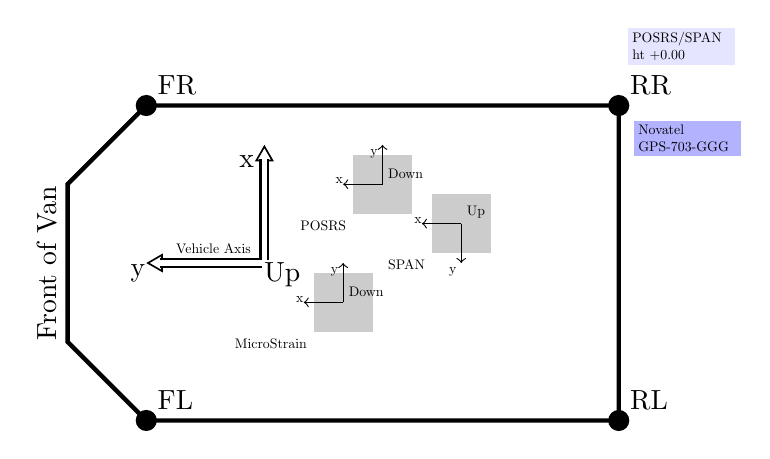
\begin{tikzpicture} [ultra thick]

%point locations
\coordinate (FR) at (2,4) ;
\coordinate (MR) at (5,4); 
\coordinate (RR) at (8,4);
\coordinate (FL) at (2,0); 
\coordinate (ML) at (5,0); 
\coordinate (RL) at (8,0); 
\coordinate (Dash) at (1,2); 
%support coordinate
\coordinate (VanCentre) at ($ (FL)!.5!(FR) + (1.5,0) $); %half way between those points

%IMU
\coordinate (POSRS) at (5.0,3.0); 
\coordinate (SPAN) at (6.0,2.5); 
\coordinate (MicroStrain) at (4.5,1.5); 

%draw points
\filldraw 
\TXT{FR}
%\TXT{MR}
\TXT{RR}
\TXT{FL}
%\TXT{ML}
\TXT{RL}
%\TXT{Dash}
;

%Van outline
\draw  (1,3) --  (1,1)  node[below,  sloped, midway,fill=white]{\rotatebox{180}{Front of Van}}
--(2,0) --(8,0)--(8,4) -- (2,4) -- cycle ;


%draw dimensions
% \begin{scope}[every node/.style={scale=0.5}, every line/.style={thin}]
% \Dims{FR}{MR}{0.815};
% 
% \end{scope}

%antena description
\tikzstyle{AntDescr} = [fill=blue!30]
\tikzstyle{AntColor} = [fill=blue!10]
\begin{scope}[every node/.style={scale=0.5},text width=2.5cm]

	%\LocationDescr{FR}{Novatel GPS-600}{Yellow}
	\LocationDescr{RR}{Novatel \\ GPS-703-GGG}{POSRS/SPAN\\ ht +0.00}
	%\LocationDescr{RR}{Novatel \\ GPS-703-GGG}{Green}
	%\LocationDescr{FL}{Novatel \\ GPS-703-GGG}{Blue}
	%\LocationDescr{FL}{Novatel \\ GPS-703-GGG}{Leica GS10\_01 ht +0.00}
	%\LocationDescr{RL}{reelekronika LORADD-A-H1 \\ LORAN+GPS}{white}
	%\LocationDescr{MR}{no antenna}{Red}
	%\LocationDescr{ML}{no antenna}{Yellow/Green stripes}
	%another dash
	%\LocationDescr{MobUser}{Centre of dash over cubby}{appox location}
 \end{scope}

%Drw wehicle axis
\VehicleAxis{VanCentre};

%IMU locations
\tikzstyle{AntDescr} = [fill=black!20]
	\IMUDescr{POSRS}{POSRS}{1}{Down}
	\IMUDescr{SPAN}{SPAN}{-1}{Up}
	\IMUDescr{MicroStrain}{MicroStrain}{1}{Down}

\end{tikzpicture}